\documentclass[10pt,a4paper, openany]{book}
\usepackage[utf8]{inputenc}
\usepackage[english]{babel}
\usepackage{amsmath}
\usepackage{amsfonts}
\usepackage{amssymb}
\usepackage{graphicx}
\usepackage{lmodern}
\usepackage[sc]{mathpazo}
\usepackage{booktabs}
\usepackage{hyperref}
\hypersetup{pdftex, colorlinks=true,linkcolor=black}

\author{Armando Brandonisio}
\title{\textbf{Absorber characterization}\\COMPASS thesis}

\begin{document}
\maketitle
\tableofcontents \newpage


\chapter{Absorber characterization}
We investigated luminescence and scintillation properties of the $Gd_3 Al_2 Ga_3 O_{12} : Ce$ (GAGG) produced by \emph{Furukawa} company. The GAGG crystal has the highest light yield among oxide crystal at room temperature \cite{abs:1} and fast decay time for the detection of radioactivity and in nuclear and particle physics experiments.\\
A list of the most important parameters for GAGG is reported in Table \ref{tab:abs1}.\\[2ex]
Some fundamental features of this crystal are that it has no intrinsic radioactivity and it is a non-hygroscopic material. This allows a better usage for experimentation with low risk of contamination from ambient.\\[2ex]
The measurements have been carried out by illuminating the scintillation rod with a X-ray beam.\\
$Si$PM and electronic chain parameters was varied measuring the relative position of the photo-peak in the spectrum produced by the scintillator.

\begin{table}[h]
\begin{tabular}{cccccccc}
\toprule
Density & Light & Decay & Peak & Energy & Hygroscopicity  \\
 $[g/cm^3]$ & yield & time & emission & resolution &   \\
   & [photon/MeV] & [ns] & [nm] & [\% @662 keV] &   \\
\midrule
6.63 & 57000 & 88 (91\%) & 520 & 5.2  & No\\
 & & 258 (9\%) & & & \\
\bottomrule
\end{tabular}
\caption{Physical and scintillation properties of GAGG} \label{tab:abs1}
\end{table}

\section{Experimental set-up}
Laboratory measurements have been carried out using a single rod made of GAGG produced by \emph{Furukawa} company.\\
The rod has a square-base parallelepipoidale shape with a height of 30mm and a side of 3mm , thus their dimension results 2/3 lower  to the one expected for the polarimeter bars ($\sim 10mm$).\\
To minimize the loss of photons during scintillation, the bar was \emph{wrapped} with Teflon Fig~\ref{fig:gagg1}, that has a high reflection coefficient for small incident angles.\\


\begin{figure}[!h]
\begin{center}
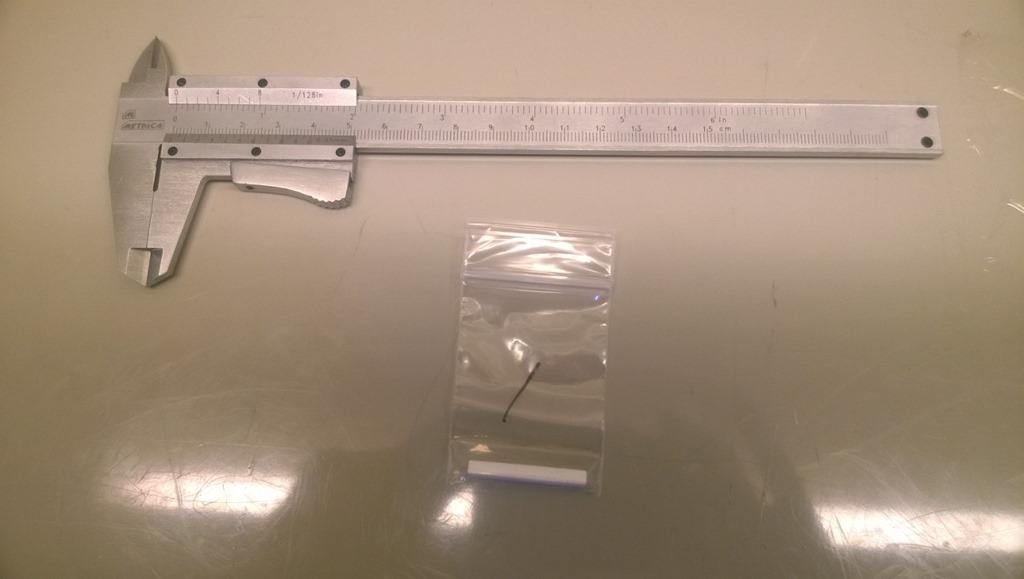
\includegraphics[scale=0.4]{imm/gagg1.jpg}
\end{center}
\caption{Scintillation rod made of GAGG wrapped with teflon}
\label{fig:gagg1}
\end{figure}

\section{Definition of the operative range}

\section{Circuit calibration with X-ray sources}

\section{Energy resolution measurement}

\clearpage
\addcontentsline{toc}{chapter}{\refname}
\begin{thebibliography}{20}

\bibitem{abs:1}
Hye-Lim Kim et al. Journal of Ceramic Processing Research. Vol. 16, No. 1, pp. 124-128, 2015

\end{thebibliography}
\end{document}
